\[
	{\small   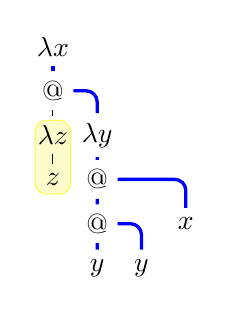
\begin{tikzpicture}[auto, scale = 0.75]
		%%%%%%%%%%%%%
		\filldraw[fill = yellow!20, draw = yellow!70, rounded corners] (-0.3, -1.25) rectangle (0.3, -2.5);
		%\filldraw[fill = yellow!20, draw = yellow!70, rounded corners] (0.45, -2.75) rectangle (1.75, -4);
		%%%%%%%%%%%%%
		\node (a) at (0, 0) {$\lambda x$};
		\node (b) at (0, -0.75) {$@$};
		\node (c) at (0, -1.5) {$\lambda z$};
		\node (d) at (0, -2.25) {$z$};
		\node (e) at (0.75, -1.5) {$\lambda y$};
		\node (f) at (0.75, -2.25) {$@$};
		\node (g) at (0.75, -3) {$@$};
		\node (h) at (0.75, -3.75) {$y$};
		\node (i) at (1.5, -3.75) {$y$};
		\node (j) at (2.25, -3) {$x$};
		%%%%%%%%%%%%%
		\draw [very thick, blue] (a) to (b);
		\draw (b) to (c);
		\draw (c) to (d);
		\draw [rounded corners, blue, very thick] (b) -| (e);
		\draw [blue, very thick] (e) to (f);
		\draw [very thick, blue] (f) to (g);
		\draw [blue, very thick, rounded corners] (f) -| (j);
		\draw [blue, very thick] (g) to (h); \draw [rounded corners, blue, very thick] (g) -| (i);
		%%%%%%%%%%%%%%
	\end{tikzpicture}}
\hspace{1cm}
	{\small  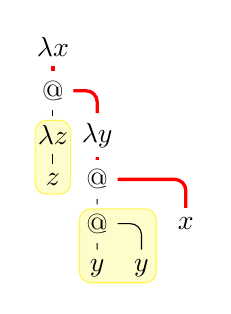
\begin{tikzpicture}[auto, scale = 0.75]
		%%%%%%%%%%%%%
		\filldraw[fill = yellow!20, draw = yellow!70, rounded corners] (-0.3, -1.25) rectangle (0.3, -2.5);
		\filldraw[fill = yellow!20, draw = yellow!70, rounded corners] (0.45, -2.75) rectangle (1.75, -4);
		%%%%%%%%%%%%%
		\node (a) at (0, 0) {$\lambda x$};
		\node (b) at (0, -0.75) {$@$};
		\node (c) at (0, -1.5) {$\lambda z$};
		\node (d) at (0, -2.25) {$z$};
		\node (e) at (0.75, -1.5) {$\lambda y$};
		\node (f) at (0.75, -2.25) {$@$};
		\node (g) at (0.75, -3) {$@$};
		\node (h) at (0.75, -3.75) {$y$};
		\node (i) at (1.5, -3.75) {$y$};
		\node (j) at (2.25, -3) {$x$};
		%%%%%%%%%%%%%
		\draw [very thick, red] (a) to (b);
		\draw (b) to (c);
		\draw (c) to (d);
		\draw [rounded corners, red, very thick] (b) -| (e);
		\draw [red, very thick] (e) to (f);
		\draw (f) to (g);
		\draw [red, very thick, rounded corners] (f) -| (j);
		\draw (g) to (h); \draw [rounded corners] (g) -| (i);
		%%%%%%%%%%%%%%
	\end{tikzpicture}}
\hspace{1cm}
	\raisebox{2cm}{
	\begin{tabular}{l c}
		{\small Spine} &
		 \raisebox{0.1cm}{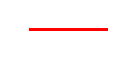
\begin{tikzpicture}[auto]
			\draw [red, very thick] (0, 0) to (1, 0);
		\end{tikzpicture}}  \\[0.2cm]
		{\small Skeleton} & {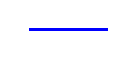
\begin{tikzpicture}[auto]
			\draw [blue, very thick] (0, 0) to (1, 0);
		\end{tikzpicture}} \\[0.2cm]
		{\small Subterm} &
		 \raisebox{-0.1cm}{
\begin{tikzpicture}[auto]
			\filldraw[fill = yellow!20, draw = yellow!70, rounded corners] (0, 0) rectangle (0.5, 0.5);
		\end{tikzpicture}}
	\end{tabular}}
\]


%
%\scalebox{0.5}{
%\[
%{ \drv{\drv[yellow]{\drv[red]{A;|;B};-[r];\drv[red!50!blue]{C;|;D}};.;\drv[blue]{D;|;E}~}}
%=
%{\drv{\drv[red]{A;|;B};-[r];\drv[yellow]{~\drv[red!50!blue]{C;|;D}~;.;\drv[blue]{D;|;E}}}}
%\]
%}

%End-of-scope markers in the $\lambda$-calculus have been seen throughout literature. \emph{Berkling's lambda bar} \cite{berkling1976symmetric} has shown to remove the need for variable names while maintaining correctness; improving efficiency by removing the need for alpha conversion \cite{BERKLING198289}. This result was generalized by \emph{Adbmal} (invert of ``Lambda'') \cite{hendriks2003lambda}. It was shown by using multiple variables, scopes can be sequenced rather than nested which correspond closely to the boxes in MELL proof nets of linear logic \cite{Lafont94fromproof-nets}. This approach was studied further in \cite{van2004lambdascope} as graph reduction that satisfies optimality \cite{levy1980optimal}. Although these approaches could identify the skeleton of a term, none however identify the spine of a term, which meant the scopes explicitly displayed may be larger than necessary from the perspective of performing substitution. This problem was solved by \emph{director strings}, introduced by Kennaway and Sleep in \cite{kennaway1988director} for combinator reduction and then generalized for any strategy by Fern\'{a}ndez et al.\ in \cite{fernandez2005lambda}. Director strings are an annotation on terms detailing the location of variable occurrences. An apt annotation on the body of an abstraction will consequently identify the spine of it. Despite being implementations that use director strings \cite{sinot2003efficient, fernandez2005lambda, fernandez2005closed}, an implementation with sharing techniques allowing for duplicating solely the spine could not be found.




%\end{document}

%We investigate the computational meaning of the following \emph{switch} rule of deep-inference proof theory \cite{Tiu:06:A-System:ai, Guglielm07}:
%\begin{center}
%	\drv{(A \rightarrow B) \wedge C ; -[s] ; A \rightarrow (B \wedge C)}
%\end{center}
%On its own, it corresponds to an \emph{end-of-scope} marker in $\lambda$-calculus. This is a special annotation of a subterm, to indicate that a given variable does not occur free, so that a substitution on that variable can be aborted early. In the above rule, $A$ corresponds to the binding variable of an abstraction and $C$ to the subterm of said abstraction where it doesn't occur, while $B$ represents those subterms where it does occur.
%
%The main thrust of our work is to incorporate this rule, and its computational interpretation as a term construct, into the \emph{atomic $\lambda$-calculus} \cite{gundersen2013atomic}. This calculus results from an investigation of the following \emph{medial} rule:
%\begin{center}
%	\drv{(A \vee B) \rightarrow (C \wedge D) ; -[m] ; (A \rightarrow C) \wedge (B \rightarrow D)}
%\end{center}
%The medial rule enables duplication to proceed \emph{atomically}: on individual constructors (abstraction and application) rather than entire subterms. The atomic $\lambda$-calculus implements \emph{full laziness}, a standard notion of sharing where only the \emph{skeleton} of a term needs to be duplicated. Given a term $t$ which needs to be duplicated, full laziness allows to share all maximal subterms $u_{1}$, . . . , $u_{k}$ of $t$ that do not contain occurrences of a variable bound in $t$ outside $u_{i}$. The constructors in $t$ not in any $u_{i}$ are then part of the skeleton.
%
%Our investigation is then focused on the interaction of switch and medial. Based on this we develop the \emph{spinal atomic $\lambda$-calculus}, a natural evolution of the atomic $\lambda$-calculus. The new calculus improves on full laziness with \emph{spinal full laziness}, which duplicates the \emph{spine} rather than the skeleton. The spine of an abstraction are the direct paths from the binder to bound variables \cite{Balabonski12}. The graph below provides an example of this for the term $\lambda x . (\lambda z . z) \lambda y . (y y) x$, where the spine of $\lambda x$ is the very thick red line and the largest subterms that could be identied by an end-of-scope operator in the term calculus (or the switch rule in the proof theory) are enclosed by yellow boxes. %would be identified by an end-of-scope operator/the switch rule are enclosed by yellow boxes.
%
%
%
%\noindent In Section \ref{sec:typingacalculus} introduces a simple sharing calculus that we expand on in Section \ref{chap:salc}, where we introduce the syntax and semantics of the spinal atomic $\lambda$-calculus, and its typing system. In Section \ref{chap:snosr} we further study the reduction rules that allow for spinal duplication, and prove natural properties of these rules such as termination and confluence. In Section \ref{chap:posn} we extend these results to include beta reduction, and show preservation of strong normalisation with respect to the $\lambda$-calculus. We conclude in Section \ref{chap:conc}.
%
%\subsection{Alternative Introduction}
%
%The \emph{scope} of an abstraction $\lambda x . M$ in the $\lambda$-calculus implicitly extends the whole of $M$. When performing a substitution $M \{N / x\}$, the substitution will traverse the whole term $M$. By making the scope explicit, we can trim the traverse space of the substitution. If there is a subterm $P$, and we know the variable $x$ does not occur freely, then we can explicitly move it out of the scope of the abstraction $\lambda x . M$ and the substitution will not needlessly traverse through $P$.
%
%\subsection{Related Work}
%
%Spine duplication has been implemented by Blanc et al.\ in \cite{blanc2007sharing}, by making use of labels in a dag-implementation. The main purpose of their work is to study sharing in Wadsworth's \emph{weak $\lambda$-calculus} \cite{wadsworth1971semantics} (further studied in \cite{CAGMAN1998239}). Balabonski \cite{Balabonski12} showed that spine duplication allows for an optimal reduction in the sense of L\'{e}vy \cite{levy1980optimal} for \emph{weak reduction} i.e.\ where a $\beta$-reduction $(\lambda x . t) s$ occurring in a subterm $u$ can only reduce if all free variables in the redex are also free in the term $u$. Blelloch and Greiner \cite{Blelloch:1995:PSF:224164.224210} showed that the weak call-by-value reduction strategy can be implemented in polynomial time with respect to the size of the initial term and the number of $\beta$ steps in said term. Given the restriction that $u$ is a closed term, this is then the same as \emph{closed reduction} \cite{fernandez1999closed, fernandez2005closed}. Our work generalizes spine duplication to the $\lambda$-calculus. It uses environments to implement sharing, and does not make use of labels, while maintaining a close intuition to dag-implementations.
%
%End-of-scope markers in the $\lambda$-calculus have been seen throughout literature. \emph{Berkling's lambda bar} \cite{berkling1976symmetric} has shown to remove the need for variable names while maintaining correctness; improving efficiency by removing the need for alpha conversion \cite{BERKLING198289}. This result was generalized by \emph{Adbmal} (invert of ``Lambda'') \cite{hendriks2003lambda}. It was shown by using multiple variables, scopes can be sequenced rather than nested which correspond closely to the boxes in MELL proof nets of linear logic \cite{Lafont94fromproof-nets}. This approach was studied further in \cite{van2004lambdascope} as graph reduction that satisfies optimality \cite{levy1980optimal}. Although these approaches could identify the skeleton of a term, none however identify the spine of a term, which meant the scopes explicitly displayed may be larger than necessary from the perspective of performing substitution. This problem was solved by \emph{director strings}, introduced by Kennaway and Sleep in \cite{kennaway1988director} for combinator reduction and then generalized for any strategy by Fern\'{a}ndez et al.\ in \cite{fernandez2005lambda}. Director strings are an annotation on terms detailing the location of variable occurrences. An apt annotation on the body of an abstraction will consequently identify the spine of it. Despite being implementations that use director strings \cite{sinot2003efficient, fernandez2005lambda, fernandez2005closed}, an implementation with sharing techniques allowing for duplicating solely the spine could not be found.


%\begin{figure}[h]
%	\centering
%	\begin{subfigure}[b]{0.3\textwidth}
%{ \small
%\drv{X ; | ; Z} {:}{:}{=} $a$ $\vert$ \drv{\drv[yellow]{X_{1} ; | ; Z_{1}} * \drv[yellow]{X_{1} ; | ; Z_{1}}} $\vert$ \drv{\drv[yellow]{X ; | ; Y_{1}} ; -[r] ; \drv[yellow]{Y_{2} ; | ; Z}}
%}
%	\caption{Derivations}
%	\label{fig:derivations}
%	\end{subfigure}
%	\hfill
%	\begin{subfigure}[b]{0.6\textwidth}
%{ \small
%\drv{\drv[yellow]{X ; | ; Y} ; . ; \drv[yellow]{Y ; | ; Z}} ~{:}{=}~ \drv{X ; . ; \drv[yellow]{X ; | ; Z}} $=$ \drv{\drv[yellow]{X ; | ; Z} ; . ; Z} $=$ \drv{X ; | ; Z}
%} \hfill
%{\small
%\drv{ \drv[yellow]{\drv[magenta]{X_{1} ; | ; Y_{1}} * \drv[orange]{X_{2} ; | ; Y_{2}}} ; . ; \drv[yellow]{\drv[cyan]{Y_{1} ; | ; Z_{1}} * \drv[green]{Y_{2} ; | ; Z_{2}}}}
%=
%\drv{\drv[yellow]{ \drv[magenta]{X_{1} ; | ; Y_{1}} ; . ; \drv[cyan]{Y_{1} ; | ; Z_{1}}} * \drv[yellow]{ \drv[orange]{X_{2} ; | ; Y_{2}} ; . ; \drv[green]{Y_{2} ; | ; Z_{2}} }}
%}
%	\caption{Vertical composition}
%	\label{fig:vertical}
%	\end{subfigure}
%%\caption{Derivations and Vertical Composition}
%%\label{fig:dervandcomp}
%\end{figure}


%Deep inference is a methodology for designing proof systems. Inference rules in deep inference, such as switch and medial, can be applied `deeply' i.e.\ there is no concept of the main connective of a formula. The \emph{open deduction} formalism \cite{opendeduction10} is designed around this principle, where logical connectives can be applied at the level of derivations as well as formulae. A derivation from premise $A$ to conclusion $C$ (over the connectives conjunction and implication) is constructed as follows,
%\begin{definition}
%A \emph{derivation} in open deduction is defined as follows.
%\begin{center}
%\drv{A ; | ; C}
%\hspace{0.5cm}
%::=
%\hspace{0.5cm}
%\drv{A}
%\hspace{0.2cm}
%$\vert$
%\hspace{0.2cm}
%\drv{\drv{A_{1} ; | ; C_{1}} \wedge \drv{A_{2} ; | ; C_{2}}}
%\hspace{0.2cm}
%$\vert$
%\hspace{0.2cm}
%\drv{\drv{C_{1} ; | ; A_{1}} \rightarrow \drv{A_{2} ; | ; C_{2}}}
%\hspace{0.2cm}
%$\vert$
%\hspace{0.2cm}
%\drv{A ; | ; B_{1} ; -[r] ; B_{2} ; | ; C}
%\end{center}
%\end{definition}
%
%\noindent where from left to right, (1) the premise and the conclusion can be the same formula i.e. $A = C$. (2) We can compose derivations horizontally with a conjunction $\wedge$, where $A = A_{1} \wedge A_{2}$ and $C = C_{1} \wedge C_{2}$. (3) We can compose derivations horizontally with an implication $\rightarrow$ where $A = A_{1} \rightarrow A_{2}$ and $C = C_{1} \rightarrow C_{2}$. Note that the derivation on the antecedent of the implication is inverted; it can be interpreted as a derivation where we treat the premise as the conclusion and the conclusion as the premise. Lastly (4) derivations can be composed vertically with an inference rule $r$ from $B_{1}$ to $B_{2}$. We work modulo symmetry, associativity, and unit laws of conjunction. Additionally the generic vertical composition of two derivations (without a mediating rule) exists as a derived operation in \cite{opendeduction10}.
%
%Open deduction was used to type the \emph{basic calculus}, which was introduced in \cite{gundersen2013atomic} as a basis for the atomic $\lambda$-calculus. We follow the same approach here; we reintroduce the basic calculus and show its typing system can be extended with the switch rule, and later expand on this to introduce the spinal atomic $\lambda$-calculus. We obtain a formulation of minimal logic together with the switch rule, from embedding its usual natural deduction system into open deduction. The rules are (respectively) called abstraction, switch, application and ($n$-ary) contraction from left to right.
%\begin{center}
%\drv{\top ; -[\lamrule] ; A \rightarrow A}
%\hspace{0.5cm}
%\drv{(A \rightarrow B) \wedge C ; -[s] ; A \rightarrow (B \wedge C)}
%\hspace{0.5cm}
%\drv{A \wedge (A \rightarrow B) ; -[\apprule] ; B}
%\hspace{0.5cm}
%\drv{A ; -[\sharerule] ; A \wedge \dots \wedge A}
%\end{center}
%These rules are used to type terms of the \emph{basic calculus}, given by the grammar
%\begin{definition}
%\label{def:basiccalc}
%\quad $s, t \quad {:}{:}{=} \quad x \quad \vert \quad \abs{x}{t} \quad \vert \quad \app{s}{t} \quad \vert \quad \share{s}{x_{1}, \dots, x_{n}}{t}$
%\end{definition}
%where the four constructors are called, from left to right, variable, abstraction, application and sharing. This is a \emph{linear} calculus, so each variable occurs at most once, and a sharing construct is used to represent multiple occurrences of a variable (or term). The variable bound by an abstraction must occur within the body of the abstraction i.e.\ in the term $\abs{x}{t}$, $x \in \fv{t}$. Lastly and similarly, each variable bound by the sharing construct must occur and become bound i.e.\ in the term $\share{s}{x_{1}, \dots, x_{n}}{t}$, each $x_{i} \in \fv{u}$ for all $1 \leq i \leq n$.
%
%
%For a given set $\set{a, b, c, \dots}$ of \emph{atomic formulae}, the following two grammars define \emph{minimal formulae} and \emph{conjunctive formulae} respectively.
%
%\begin{center}
%$A, B, C \quad {:}{=} \quad a \, \, \, \vert \, \, \, A \rightarrow B$ \hspace{1cm} $\Gamma, \Delta \quad {:}{=} \quad A \, \, \, \vert \, \, \, \top \, \, \, \vert \, \, \, \Gamma \wedge \Delta$
%\end{center}
%
%The typing derivations in open deduction for this calculus is displayed in Figure \ref{fig:typebasic}, where the corresponding types and derivations for terms are in red. We add the boxes to aid the reader see the horizontal composition of derivations. The colour of the box has no meaning other than to help identify derivations. A variable $x$ may be typed by any minimal formula $A$, while the other constructors each correspond to inference rules, used within the context of further derivations. A term $t$ with free variables $x_{1}, \dots, x_{n}$ can be typed by a derivation from assumption $A_{1}^{{\color{red} x_{1}}} \wedge \dots \wedge A_{n}^{{\color{red} x_{n}}}$ to conclusion $C$. A \emph{typing judgement} $t : C$ then expresses that $t$ is typeable by a derivation with conclusion $C$. Note that a derivation occurring as the antecedent of an implication is always a minimal formula.
%
%\begin{figure}[h]
%\begin{center}
%\begin{tabular}{c c c c}
%\drv{A^{\color{red} x}}
%\hspace{0.2cm}
%&
%\drv{ \drv[yellow]{\top ; -[\lamrule] ; A \rightarrow A} \wedge \Gamma ; -[s] ; A \rightarrow \drv[green]{A^{\color{red} x} \wedge \Gamma ; |[\color{red} t] ; B}}
%\hspace{0.2cm}
%&
%\drv{\drv[yellow]{\Gamma ; |[\color{red}s] ; A} \wedge \drv[yellow]{\Delta ; |[\color{red}t] ; A \rightarrow B} ; -[\apprule] ; B}
%\hspace{0.2cm}
%&
%\drv{\drv[yellow]{ \Delta \wedge \drv[green]{\Gamma ; |[\color{red} t] ; A ; -[\sharerule] ; A^{\color{red} x_{1}} \wedge \dots \wedge A^{\color{red} x_{n}}}} ; |[\color{red} s ] ; B}
%\end{tabular}
%\end{center}
%\caption{Typing derivations for terms in the basic calculus}
%\label{fig:typebasic}
%\end{figure}
%
%%The terms can also be interpreted graphically, as displayed below. Notice that the derivations are rotated 180 degrees compared to the graphical depictions of the terms.
%%\begin{center}
%%\begin{tabular}{c c c c}
%%{\begin{tikzpicture}[AL]
%% \draw [->] (0,1) -- (0,-1) ;
%%\end{tikzpicture}}
%%\hspace{0.2cm}
%%&
%% Lambda
%%{\begin{tikzpicture}[AL]
%% \ALnodeL{0,0}a;
%% \ALnodeT[.5]t{0,-1.5}t;
%% \draw [<-] (a_1) -- (0,1);
%% \draw [->] (a_2) -- (t_top);
%% \draw [<-,rounded corners] (a_3) -- (1,0) -- (1,-2.5) -| (0.25, -2.1);
%% \draw [->] (-0.25, -2.1) -- (-.25, -3.5);
%%\ALbar{(-.25,-2.6)};
%%\end{tikzpicture}}
%%\hspace{0.2cm}
%%&
%% Application
%%{\begin{tikzpicture}[AL]
%% \path (0,1) (0,-2.5);
%% \ALnodeA{0,0}a;
%% \ALnodeT[.5]s{0,-1.5}s;
%% \ALnodeT[.5]t{1.2,-1.5}t;
%% \draw [<-] (a_1) -- (0,1);
%% \draw [->] (a_2) -- (s_top);
%% \draw [->,rounded corners] (a_3) -| (t_top);
%% \draw [->] (t_bot) -- +(0pt, -10pt);
%% \ALbar{(t_bot) ++(0pt, -5pt)};
%% \draw [->] (s_bot) -- +(0pt, -10pt);
%% \ALbar{(s_bot) ++(0pt, -5pt)};
%%\end{tikzpicture}}
%%\hspace{0.2cm}
%%&
%% Sharing
%% {\begin{tikzpicture}[AL]
%% \ALnodeT[1.5]s{0,1.5}s;
%% \draw [->] (-0.7, .9) -- (-0.7, -3);
%% \ALbar{(-.7, -1)};
%% \begin{scope}[xshift = 5pt]
%% \ALnodeS{0,0}v;
%%\ALnodeT[.5]t{0,-1.5}t;
%% \draw [->] (s_bot -| v_left) -- (v_left);
%% \draw [->] (s_bot -| v_right) -- (v_right);
%% \draw [->] (v_tip) -- (t_top);
%% \ALdots{0,0.6};
%% \draw [->] (0, -2.1) -- (0, -3);
%% \ALbar{(0, -2.55)};
%%\end{scope}
%%\end{tikzpicture}}
%%\end{tabular}
%%\end{center}
%
%\noindent The semantics of the basic calculus, including the compilation and readback into the $\lambda$-calculus, can be found in \cite{gundersen2013atomic} and will not be repeated here.
%
%Although in the derivation for an abstraction in Figure \ref{fig:typebasic} we place the switch rule directly after the abstraction rule, this is not always the case. Consider the term $t = \lambda x . \lambda y . x y$, where $x : A \rightarrow B =  C$ and $y : A$. The following derivations are both typing judgements of $t : C \rightarrow A \rightarrow B$.
%\begin{center}
%\drv{\top ; -[\lamrule] ; C \rightarrow \drv[green]{C \wedge \drv[yellow]{\top ;-[\lamrule] ; A \rightarrow A} ; -[s] ; A \rightarrow \drv[magenta]{C \wedge A ; -[\apprule] ; B}}}
%\hspace{0.5cm}
%$\sim$
%\hspace{0.5cm}
%\drv{ \drv{\top ; -[\lamrule] ; C \rightarrow C} \wedge \drv[yellow]{\top ; -[\lamrule] ; A \rightarrow A} ; -[s] ; C \rightarrow \drv[green]{C \wedge (A \rightarrow A) ; -[s] ; A \rightarrow \drv[magenta]{C \wedge A ; -[\apprule] ; B}}}
%\end{center}
%
%The main difference between the two is that the first is \emph{scope-balanced} while the second is \emph{unbalanced} (terminology taken from \cite{hendriks2003lambda}). In derivations, the \emph{scope} of an abstraction is considered to be the subderivation found underneath the corresponding switch rule. In the scope-balanced derivation, the scope of the binder $\lambda x$ is the whole body of the term; any scopes of any binders underneath $\lambda x$ (such as $\lambda y$) are considered nested within the scope of $\lambda x$. The scope of an abstraction in the scope-balanced derivation corresponds to the skeleton of the term. In the unbalanced derivation, scopes are not strictly nested but can overlap. The variable $y$ (with type $A$) is now identified by the switch rule corresponding with $\lambda x$, and is not considered within the scope of $\lambda x$ in contrast to the balanced derivation where is was nested. The unbalanced scope of an abstraction corresponds with the spine of the term. Both derivations identify the application in all scope.
%
%%\begin{center}
%%{\color{red} Add a picture here highlighting the scopes? Should I be general or use the specific example}
%%\end{center}
%
%The atomic $\lambda$-calculus can be seen as using only scope-balanced derivations, and here we show that by using unbalanced derivations we can identify the spine of an abstraction, and moreover when introducing the medial rule to the typing system duplicate said spine by proof normalisation.
%%
%%We iterate the point here that the switch rule corresponds to an end-of-scope marker in the $\lambda$-calculus. To understand the idea, consider a closed term $\lambda x . t$ with $n$ maximal subterms $s_{1}, \dots, s_{n}$ that do not contain $x$ as a free variable. This abstraction can then be typed with the following derivation, where the derivation of $t$ is the composition of the derivations of each subterm $s_{i}$ as well as the derivation of the spine of $t$. It is possible to use a switch rule to mark each subterm independently, resulting in a possible explicit end-of-scope marker in the term calculus, but we choose to simplify such that each abstraction rule has at most one switch rule.
%%
%%\begin{center}
%%\drv{\drv[yellow]{\top ; -[\lamrule] ; A \rightarrow A^{\color{red} x}} \wedge \drv{\top ; |[{\color{red} s_{1}}] ; B_{1}} \wedge \dots \wedge  \drv{\top ; |[{\color{red} s_{n}}] ; B_{n}} ; -[s] ; A \rightarrow \drv[green]{A \wedge B_{1} \wedge \dots \wedge B_{n} ; |[{\color{red} t-spine}] ; C}}
%%\end{center}


%We extend the basic calculus with a new construct, based of the medial inference rule.  In classical logic, the medial rule is the key to reducing contractions to their atomic case during proof normalisation \cite{BrunTiu:01:A-Local-:mz}. This result also translates into intuitionistic logic, and is the key factor to allowing atomic reduction. The medial rule studied in \cite{gundersen2013atomic} uses disjunction, and to avoid introducing disjunction into the typing system the authors instead use the following \emph{distribution rule}, which combines the medial with a co-contraction rule (the reversed contraction rule that works with disjunction rather than conjunction).
%\begin{center}
%	\drv{A \rightarrow (B \wedge C) ; -[d] ; (A \rightarrow B) \wedge (A \rightarrow C)}
%\end{center}
%The distribution rule is introduced when an abstraction meets a contraction rule. The proof reduction step to be implemented in the spinal atomic $\lambda$-calculus is as follows.
%\begin{center}
%\drv{(A \rightarrow A) \wedge \Gamma ; -[s] ; A \rightarrow \drv[yellow]{A \wedge \Gamma ; | ; B} ; -[\sharerule] ; (A \rightarrow B) \wedge (A \rightarrow B)}
%\hspace{0.5cm}
%$\rightsquigarrow$
%\hspace{0.5cm}
%\drv{(A \rightarrow A) \wedge \Gamma ; -[s] ; A \rightarrow \drv{\drv[yellow]{A \wedge \Gamma ; | ; B} ; -[\sharerule] ; B \wedge B} ; -[d] ; (A \rightarrow B) \wedge (A \rightarrow B)}
%\end{center}
%
%By doing this, we leave a contraction applied to a subderivation for a term $\lambda x . t$. This reduction step allows to push the contraction past the abstraction, inside the body $t$, without duplicating any part of $t$ itself. The abstraction $\lambda x$ becomes duplicated, creating \emph{phantom-abstractions} (the derivations that occur underneath the distributor). Phantom-abstractions can intuively be interpretated as partially duplicated abstractions. The idea is that the contraction continues to duplicate $t$ stepwise, and the copies gets substituted into the body of the phantom-abstractions, i.e.\ subderivations produceed by continuing the duplication of $t$ are moved underneath the distributor rule as shown in Figure \ref{fig:flush}.
%\begin{figure}[h]
%\begin{center}
%\drv{(A \rightarrow A) \wedge \Gamma ; -[s] ; A \rightarrow \drv[yellow]{A \wedge \Gamma ; | ; C ; -[\sharerule] ; \drv[green]{C ; | ; B} \wedge \drv[green]{C ; | ; B}} ; -[d] ; (A \rightarrow B) \wedge (A \rightarrow B)}
%\hspace{0.5cm}
%$\rightsquigarrow$
%\hspace{0.5cm}
%\drv{(A \rightarrow A) \wedge \Gamma ; -[s] ; A \rightarrow \drv[yellow]{A \wedge \Gamma ; | ; C ; -[\sharerule] ; C \wedge C} ; -[d] ; (A \rightarrow \drv[green]{C ; | ; B}) \wedge (A \rightarrow \drv[green]{\Delta ; | ; B})}
%\end{center}
%\caption{Flushing terms through the distributor}
%\label{fig:flush}
%\end{figure}
%
%As the duplication of the body of the abstraction proceeds we may create contraction rules on derivations that do not contain the bound variable. Instead of duplicating, we can instead `lift' the derivation outside the scope of the abstraction. This is implemented in the following proof reduction step.
%\begin{center}
%\drv{(A \rightarrow A) \wedge \Gamma_{1} \wedge \Gamma_{2} ; -[s] ; A \rightarrow \drv[yellow]{\drv[green]{A \wedge \Gamma_{1} ; | ; C \wedge C} \wedge \drv[magenta]{\Gamma_{2} ; | ; D \wedge D}} ; -[d] ; (A \rightarrow C \wedge D) \wedge (A \rightarrow C \wedge D)}
%\hspace{0.5cm}
%$\rightsquigarrow$
%\hspace{0.5cm}
%\drv{(A \rightarrow A) \wedge \Gamma_{1} \wedge \drv[magenta]{\Gamma_{2} ; | ; D \wedge D} ; -[s] ; A \rightarrow \drv[yellow]{\drv[green]{A \wedge \Gamma_{1} ; | ; C \wedge C} \wedge D \wedge D} ; -[d] ; (A \rightarrow C \wedge D) \wedge (A \rightarrow C \wedge D)}
%\end{center}
%
%\noindent After lifting the derivation, we may notice that the formula $D$ does not need to be affiliated with the switch rule but instead can be directly placed using switch rules on the phantom-abstractions. As we are duplicating an abstraction, the partially duplicated abstractions will also have scopes and it is natural that they would also have switch rules that maintain these scopes during duplication. The derivation we lift is not considered part of the spine, and by placing a switch rule on the phantom-abstraction we are transferring this information to the copies of the abstraction. Thus the spine of the copies are equal to the spine of the original.
%\begin{center}
%\drv{(A \rightarrow A) \wedge \Gamma_{1} \wedge \drv[magenta]{\Gamma_{2} ; | ; D \wedge D} ; -[s] ; A \rightarrow \drv[yellow]{\drv[green]{A \wedge \Gamma_{1} ; | ; C \wedge C} \wedge D \wedge D} ; -[d] ; (A \rightarrow C \wedge D) \wedge (A \rightarrow C \wedge D)}
%\hspace{0.5cm}
%$\rightsquigarrow$
%\hspace{0.5cm}
%\drv{\drv[cyan]{(A \rightarrow A) \wedge \Gamma_{1} ; -[s] ; A \rightarrow \drv[green]{A \wedge \Gamma_{1} ; | ; C \wedge C} ; -[d] ; (A \rightarrow C) \wedge (A \rightarrow C)} \wedge \drv[magenta]{\Gamma_{2} ; | ; D \wedge D} ; =[s] ; (A \rightarrow C \wedge D) \wedge (A \rightarrow C \wedge D)}
%\end{center}
%Eventually all the free variables affiliated with the switch are passed to the phantom-abstractions, and the switch rule associated with the abstraction being duplicated will be redundant. If we move all other derivations out of the distribution scope by lifting and flushing as shown in Figure \ref{fig:flush}, eventually the distribution rule will meet the abstraction rule. The distribution inference can then be eliminated by the reduction step below.
%\begin{center}
%\drv{\top ; -[\lambda] ; A \rightarrow \drv{A ; -[\sharerule] ; A \wedge A} ; -[d] ; (A \rightarrow A) \wedge (A \rightarrow A)}
%\hspace{0.5cm}
%$\rightsquigarrow$
%\hspace{0.5cm}
%\drv{\drv{\top ; -[\lambda] ; A \rightarrow A} \wedge \drv{\top ; -[\lambda] ; A \rightarrow A}}
%\end{center}
%
%To implement reductions of this kind, we extend the basic calculus (Definition \ref{def:basiccalc}) with two new constructs, the \emph{distributor} that corresponds to the distribution inference and \emph{phantom-abstractions} that correspond to the partially duplicated abstractions.


%\noindent Below we show some examples of pre-terms and terms
%
%\begin{itemize}
%	\item Pre-Terms (not Terms)
%
%\begin{itemize}
%	\item $\fake{c}{x}{y}$.
%
%	Violating condition $3$ in Definition \ref{def:falcterms}.
%	\item $\share{\app{x}{y}}{x, z}{w}$.
%
%	Violating condition $4$
%	\item $\app{\fake{e_{2}}{w_{2}}{w_{2}}}{(\app{(\fake{e_{1}}{w_{1}}{w_{1}})}{z})} \dist{}{\fakedist{e_{1}}{w_{1}}, \fakedist{e_{2}}{w_{2}}}{\share{}{w_{1}, w_{2}}{\fake{x}{x}{\app{x}{y}}}}{c}{z}$
%
%	Violating condition $6(b)$
%\end{itemize}
%	\item Terms
%\begin{itemize}
%	\item $\fake{x}{x}{x}$
%	\item $\fake{x}{x}{(\fake{y}{y}{\share{\app{x_{1}}{(\app{x_{2}}{y})}}{x_{1}, x_{2}}{x}})}$
%	\item $ \app{\fake{e_{2}}{w_{2}}{w_{2}}}{(\app{(\fake{e_{1}}{w_{1}}{w_{1}})}{z})} \dist{}{\fakedist{e_{1}}{w_{1}}, \fakedist{e_{2}}{w_{2}}}{\share{}{w_{1}, w_{2}}{\fake{x}{x}{\app{x}{c}}}}{c}{c}$
%\end{itemize}
%\end{itemize}


%The terms typed by the derivations in Figure \ref{fig:typebasic} and Figure \ref{fig:derivphandist}. Figure \ref{fig:derivphandist} shows the derivations for the terms $\fake{d}{\vec{x}}{t}$ and $\dist{u}{\fakedist{e_{1}}{\vec{x_{1}}} \dots \fakedist{e_{n}}{\vec{x_{n}}}}{\overline{[\Gamma]}}{c}{c}$. The distributor construct is typed using the medial rule as in \cite{gundersen2013atomic}. Notice that the medial rule in Figure \ref{fig:derivphandist} does not use disjunction compared to the medial rule in the introduction. In the derivation we combine the medial rule with a co-contraction rule to form the \emph{distribution rule} ($d$). Since the formula in the ante-cedent of an implication is always a minimal formula, doing this allows us to avoid introducing disjunction into the typing system.
%
%The main difference between our calculus is the bindings. We create a new class of bindings, where phantom-variables are captured by the distributor but variables are captured by the environment of the distributor. This shows in the derivations since the types of the variables ($\Sigma$ and $\Phi$) are not captured by the distribution rule.


%\noindent The distributor is illustrated below; it is depicted as a box encompassing an environment and a co-contraction.
%
%\begin{center}
%\begin{tabular}{c c}
%{\begin{tikzpicture}[AL]
%\filldraw[fill = green!30, draw = green!70, rounded corners] (-1, 0.7) rectangle (1, -3);
% \ALnodeP{0,0}a;
% \ALnodeT[.5]t{0,-1.5}t;
% \draw [<-] (a_1) -- (0,1);
% \draw [->] (a_2) -- (t_top);
% \draw [<-,rounded corners] (a_3) -- (1.5,0) -- (1.5,-2.5) -| (1.5, -3.5);
% \draw [->] (-0.25, -2.1) -- (-.25, -3.5);
%\ALbar{(-.25,-2.6)};
% \draw [->] (0.25, -2.1) -- (.25, -3.5);
%\ALbar{(.25,-2.6)};
%\node at (-0.625, -2.5) {\tiny \color{red} $\vec{x}$};
%\node at (0.625, -2.5) {\tiny \color{red} $\vec{y}$};
%\node at (1.75, -2) {\tiny \color{red} $c$};
%\end{tikzpicture}}
%&
%%%%%%%%%%%%%%
%{\begin{tikzpicture}[AL]
%\draw[rounded corners] (-2.5, 4.75) rectangle (6.5, -2.6);
% \filldraw[fill = green!30, draw = green!70, rounded corners] (-0.75, 1) rectangle (0.75, -1.85);
%\filldraw[fill = black!20, draw = black!70, rounded corners, thick] (-1, -2.8) rectangle (6.5, -5.5);
%\ALnodeP{0, 0.5}a;
% \draw[->] (-1.75, -2.6) -- (-1.75, -6);
%\draw [->] (0, 5) -- (a_1);
%\ALnodeT[.5]{}{0, -1}t;
%\draw [->] (a_2) -- (t_top);
%\ALdots{2, 4};
% \node at (0, 3) { $u$};
%\begin{scope}[yshift = 2cm]
% \filldraw[fill = green!30, draw = green!70, rounded corners] (3.25, 0.5) rectangle (4.75, -2.35);
%\ALnodeP{4, 0}b;
%\draw [->] (4, 1) -- (b_1);
%\ALnodeT[.5]{}{4, -1.5}s;
%\draw [->] (b_2) -- (s_top);
%\end{scope}
%\draw [<-, rounded corners] (b_3) -| (6, 2) -- (6, -4);
%\draw [<-, rounded corners] (a_3) -| (5, -4) ;
%\ALdots{5.5, -2};
%\ALdots{2, 1};
%\ALnodeC{5.5, -4.2}c;
%\ALnodeT[2.5]{\overline{\Gamma}}{2, -4}h;
%\draw [->] (0, -1.6) -- (0, -3.35);
%\draw [-] (4, 1.9) -- (4, 0.6);
%\draw [->] (4, 0.4) -- (4, -3.35);
%\draw [-] (-0.2, -1.6) -- (-0.2, -3.3);
%\draw [->] (-0.2, -4.7) -- (-0.2, -6);
%\ALbar{(0, -2.3)};
%\ALbar{(-0.2, -2.3)};
%\ALbar{(4, -0.6)};
%\ALbar{(3.8, -0.6)};
%\draw [->, rounded corners] (3, -4.6) |- (5, -5) -| (c_tip);
%\draw [->] (1.8, -4.6) -- (1.8, -6);
%\ALbar{(1.8, -5.1)};
%\draw [-] (3.8, 1.9) -- (3.8, 0.6);
%\draw [-] (3.8, 0.4) -- (3.8, -3.3);
%\draw [-] (3.8, -4.7) -- (3.8, -4.9);
%\draw [->] (3.8, -5.1) -- (3.8, -6);
% \node at (1.55, -2.25) {\tiny \color{red} $x^{1}_{1}, \dots, x^{1}_{k_{1}}$};
%  \node at (2.6, -0.6) {\tiny \color{red} $x^{n}_{1}, \dots, x^{n}_{k_{n}}$};
% \node at (4.7, -2.25) {\tiny \color{red} $e_{1}$};
% \node at (5.7, -1.5) {\tiny \color{red} $e_{n}$};
% \node at (5.8, -5) {\tiny \color{red} $y$};
% \ALbar{(-1.75, -4.3)};
%\end{tikzpicture}}
%\\
%$\fake{c}{\vec{x}}{t}$ &
%$\dist{u}{\fakedist{e_{1}}{x^{1}_{1} \dots x^{1}_{k_{1}}} \dots \fakedist{e_{n}}{x^{n}_{1} \dots x^{n}_{k_{n}}}}{\overline{[\Gamma]}}{y}{y}$
%\end{tabular}
%\end{center}



%Collapsing the environment to a collection of substitutions $\sigma$ means we need to perform the substitutions either before of after interpreting $u$, i.e.\ $\trans{u}\sigma$ or $\trans{u \sigma}$. By performing the substitutions first, we conflict with condition $1$ of Definition \ref{def:falcterms}, therefore we only have the option to first interpret $u$ and then perform substitutions. Consequently, since the binding variable of abstractions in $u$ may occur in the terms of $\sigma$, intentionally due to (3), these substitutions would not be capture-avoiding. To elaborate, let $\vec{x_{1}} = x_{1}, x_{2}$. The collapsed envorinment is expected to have two substitutions $\sub{}{M_{1}}{x_{1}}, \sub{}{M_{2}}{x_{2}} \in \sigma$ where $M_{1}, M_{2} \in \Lambda$.It is possible that in $M_{1}$ or $M_{2}$ might contain $c$ as a free variable, which is the variable bound by the abstraction in the distributor. Therefore to maintain bindings, we would need the substitutions $\sub{}{M_{i} \sub{}{e_{1}}{c}}{x_{i}}$ for $i \in [2]$.
%
%Lastly, it may be the case that the phantom-abstraction in $u$ bound by the distributor is actually a part of a second distributor in $u$, i.e.\ the subterm $\dist{u'}{\fakedist{f_{1}}{\vec{y_{1}}} \dots \fakedist{f_{m}}{\vec{y_{m}}}}{\overline{[\Gamma]}}{e_{i}}{\vec{x_{i}}}$. The cover $\fakedist{e_{i}}{\vec{x_{i}}}$ is captured by the already interpreted distributor. We will have issues if we use the same reasoning as before here, since the intended bound variable for this cover is not located in this environment but would be substituted in from the previous collapsed environment (in $\sigma$). We cannot wait for these substitutions to be performed before we can interpret this distributor without breaking linearity. The solution is to use a map that is carried with the interpreting function. This map $\sigma$ (we overload notation) allows us to directly manipulate the substitutions. For further elaboration, let $\fakedist{e_{i}}{\vec{x_{i}}} = \fakedist{e_{1}}{x_{1}, x_{2}}$ from before. We know $\sub{}{M_{1} \sub{}{e_{1}}{c}}{x_{1}}, \sub{}{M_{2} \sub{}{e_{1}}{c}}{x_{2}} \in \sigma$. We can interpret this distributor, that allows us to perform the substitutions without breaking linearity since the results are stored in the map. Consider the collapsed environment $\sigma'$. For each cover captured, e.g.\ $\fakedist{f_{1}}{\vec{y_{1}}}$, and for each $y \in \vec{y_{1}}$, there is some term $N$ such that $\sub{}{N}{y} \in \sigma'$. We can maintain variable bindings (condition 3) then simply by reading the current map $\sigma$ and adding a new substitution as done before, resulting in $\sub{}{N \sub{}{M_{1} \sub{}{e_{1}}{c} \sub{}{f_{1}}{e_{1}}}{x_{1}} \sub{}{M_{2} \sub{}{e_{1}}{c} \sub{}{f_{1}}{e_{1}}}{x_{2}}}{y}$.


%\begin{definition}
%We define a map $\sigma : V \rightarrow \Lambda$ to be an infinite set of pairs of variables and $\Lambda$-terms. Given a variable $x$, $\sigma(x) = M$ such that $(x \mapsto M) \in \sigma$ and there does not exist $N$ where $M \neq N$ and $(x \mapsto N) \in \sigma$
%\end{definition}
%
%\noindent We use the following notation to make maps more concise.
%
%\begin{notation}
%We write $\sigma = \set{x_{1} \mapsto M_{1}, \dots, x_{n} \mapsto M_{n}}$ to mean the map where for $x_{i} \in \set{x_{1}, \dots, x_{n}}$, $\sigma(x_{i}) = M_{i}$ and for $y \not\in \set{x_{1}, \dots, x_{n}}$, $\sigma(y) = y$.
%\end{notation}


%We utilise two interpretations to define the readback. Given a term $N : \Lambda$, a substitution map $S : V \rightarrow \Lambda$, and a variable-indexed renaming $R: V \rightarrow V \rightarrow$, i.e.\ for a given $x$, $R_{x} : V \rightarrow V$ is a renaming function,  we can define the interpretation $\trans{t} = (\Lambda, R)$ that interprets a spinal atomic $\lambda$ terms as a pair consisting of a $\lambda$-term and renamings, and will use the auxiliary translation $\tranclos{[\Gamma]}$ which interprets closures as a pair $(S, R)$.
%
%A renaming $R$ \emph{modifies} a substitution $S$ by $S\{R\} : V \rightarrow \Lambda$, such that $S \{ R \} (x) = S(x) \{R_{x} \}$. So if $S$ has $\sub{}{N}{x}$, then $S \{ R \}$ has $\sub{}{N \{ R_{x} \}}{x}$. Renamings $R$ and $Q$ can be \emph{composed} $R \cdot Q = R_{x} \cdot Q_{x}$ for every $x$. Renaming can be \emph{joined} as $R + Q$ if $R_{x}$ and $Q_{x}$ agree where they are both defined. We thus define the translation.
%
%\begin{align*}
%	\trans{x} &= (x, 0) \\
%	\trans{st} &= (NM, R + Q) & \trans{s} = (N, R), \trans{t} = (M, Q) \\
%	\trans{\fake{c}{\vec{x}}{t}} &= (\lambda c . N, R) & \trans{t} = (N, R) \\
%	\trans{t [\Gamma]} &= (N \{S \{R \} \}, R \cdot Q) & \trans{t} = (N, R), \tranclos{[\Gamma]} = (S, Q) \\[1cm]
%	\tranclos{\share{}{x_{1}, \dots, x_{n}}{t}} &= (\sub{}{N}{x_{1}} \dots \sub{}{N}{x_{n}}, R) & \trans{t} = (N, R) \\
%	\tranclos{\dist{}{\fakedist{e_{1}}{\vec{w_{1}}}, \dots, \fakedist{e_{n}}{\vec{w_{n}}}}{\overline{[\Gamma]}}{c}{\vec{x}}} &= (S \{ R \}, R \cdot Q) & \tranclos{\overline{[\Gamma]}} = (S, Q) \\
%	& & \text{each } R_{x} = \sub{}{e_{i}}{c} \text{ for each } x \in \vec{w_{i}}
%\end{align*}
%
%In the term calculus, we consider terms equal up to the congruence induced by the exchange of closures. Consider the term $t[\Gamma_{1}][\Gamma_{2}]$ where $[\Gamma_{1}]$ and $[\Gamma_{2}]$ are both closures. Then $t[\Gamma_{1}][\Gamma_{2}] \sim t[\Gamma_{2}][\Gamma_{1}]$ iff $[\Gamma_{2}]$ only binds variables and phantom-variables located in $t$. This equivalence is essential to the rewriting theory.
%
%\begin{proposition}
%Given $t[\Gamma_{1}][\Gamma_{2}] \sim t[\Gamma_{2}][\Gamma_{1}]$ , then $\readback{t[\Gamma_{1}][\Gamma_{2}]}{\sigma} = \readback{t[\Gamma_{2}][\Gamma_{1}]}{\sigma}$
%\end{proposition}
%\begin{proof}
%
%
%Consider $\readback{t[\Gamma_{1}][\Gamma_{2}]}{}$, the intepretation of the closure $[\Gamma_{2}]$ may generate substitutions and recapturings $\sigma_{2}$ i.e.\ $\readback{t[\Gamma_{1}][\Gamma_{2}]}{} = \readback{t[\Gamma_{1}]}{} \sigma_{2}$. Using the same reasoning we can say $\readback{t[\Gamma_{1}]}{} \sigma_{2} = \readback{t}{} \sigma_{1} \sigma_{2}$. Since the variables bound by $[\Gamma_{2}]$ are only located in $t$ and not in any term in $\sigma_{1}$, we can exchange these bundles of substitutions and recapturings i.e.\ $\readback{t}{} \sigma_{1} \sigma_{2} = \readback{t}{} \sigma_{2} \sigma_{1} = \readback{t [\Gamma_{2}] [\Gamma_{1}]}{}$
%\end{proof}


%\begin{proposition}
%\label{prop:subintrans}
%Substitution commutes with the translation in the following way
%
%$$\readbackwmap{u \sub{}{t}{x}}{\sigma}{\gamma} = \readbackwmap{u}{\sigma[x \mapsto \readbackwmap{t}{\sigma}{\gamma}]}{\gamma}$$
%\end{proposition}

%\begin{proposition}
%\label{prop:bkcomm}
%Book-keeping commutes with the translation in the following way
%
%%if $\fake{c}{y_{1}, \dots, y_{m}} \in \fc{u}$ such that $\set{x_{1}, \dots, x_{n}} \subset \set{y_{1}, \dots, y_{m}}$
%%
%%and for those $z \in \set{y_{1}, \dots, y_{m}} / \set{x_{1}, \dots, x_{n}}$, $\gamma(c) \not\in \fv{\sigma(z)}$
%%
%%or if simply $\set{x_{1}, \dots, x_{n}} \cap \fv{u} = \set{}$
%
%$$\readbackwmap{u \psub{}{x_{1}, \dots, x_{n}}{c}}{\sigma}{\gamma} = \readbackwmap{u}{\sigma}{\gamma}$$
%
%\end{proposition}
%
%\begin{proposition}
%\label{prop:exorcomm}
%Exorcisms commute with the translation in the following way
%
%%if $\fake{c}{x_{1}, \dots, x_{n}} \in \fc{u}$ or $\set{x_{1}, \dots, x_{n}} \cap \fv{u} = \set{}$
%
%$$\readbackwmap{u \exor{}{c}{x_{1}, \dots, x_{n}}}{\sigma}{\gamma} = \readbackwmap{u}{\sigma[x_{i} \mapsto c]_{i \in [n]}}{\gamma}$$
%\end{proposition}


%	\begin{tikzpicture}[auto]
%		\node (ale) at (-0.5, 0) {$\FALC$};
%		\node (bob) at (2.5, 0) {$\WEAK$};
%		\node (cat) at (1,-2) {$\Lambda$};
%		%%%%%%%%%%%%%
%		\draw [->,red] (ale) to node [black] {$\readweakwmap{-}{\sigma^{\weaksymbol}}{\gamma}$}  (bob);
%		\draw [->,blue] (bob) to node [black] {$\readbackweak{-}$}  (cat);
%		\draw [->, purple] (ale) to node [black, swap] {$\readbackwmap{-}{\sigma^{\Lambda}}{\gamma}$} (cat);
%	\end{tikzpicture}
%	&
%	\begin{tikzpicture}[auto]
%		\node (ale) at (0, 0) {$\FALC$};
%		\node (bob) at (2, 0) {$\WEAK$};
%		\node (cat) at (1,-2) {$\Lambda$};
%		%%%%%%%%%%%%%
%		\draw [->,red] (ale) to node [black] {$\composeweak{-}$}  (bob);
%		\draw [->,orange] (cat) to node [black, swap] {$\compweak{-}$}  (bob);
%		\draw [->, yellow] (cat) to node [black] {$\compile{-}$} (ale);
%	\end{tikzpicture}
%	&
%	\begin{tikzpicture}[auto]
%		\node (ale) at (0, -2) {$\Lambda$};
%		\node (bob) at (2, -2) {$\Lambda$};
%		\node (cat) at (1,0) {$\WEAK$};
%		%%%%%%%%%%%%%
%		\draw [->,black] (ale) to node [black] {$=$}  (bob);
%		\draw [->,orange] (ale) to node [black] {$\compweak{-}$}  (cat);
%		\draw [->, blue] (cat) to node [black] {$\readbackweak{-}$} (bob);
%	\end{tikzpicture}
%	\\


% Lifting a closure relates ($\weaksymbol_{1}$) and (\ref{red:liftabs}), ($\weaksymbol_{2}$) and  (\ref{red:liftappleft}), ($\weaksymbol_{3}$) and (\ref{red:liftappright}), ($\weaksymbol_{4}$) and (\ref{red:liftshare}), ($\weaksymbol_{5}$) and (\ref{red:absdup}), and duplicating a term relates ($\weaksymbol_{6}$) and (\ref{red:appdup}), and  ($\weaksymbol_{7}$) and (\ref{red:distelim}).


%\scalebox{0.8}{
%	\begin{tikzpicture}[auto]
%		\node (a1) at (0, 4) {$\FALC$};
%		\node (w1) at (2, 4) {$\WEAK$};
%		\node (l1) at (4, 4) {$\Lambda$};
%		\node (li) at (4, 2) {$\infinity$}; \node (wi) at (2, 2) {$\infinity$}; \node (ai) at (0, 2) { \color{myGreen} $\infinity$};
%		%%%%%%%%%%%%
%		\draw [->, decorate,decoration={snake,amplitude=.4mm,segment length=2mm,post length=1mm}] (l1) -> (li);
%		 \draw [->, decorate,decoration={snake,amplitude=.4mm,segment length=2mm,post length=1mm}] (w1) -> (wi);
%		 \draw [->, myGreen, decorate,decoration={snake,amplitude=.4mm,segment length=2mm,post length=1mm}] (a1) -> (ai);
%		\draw [myGreen] (-0.3, 2.75) -- (0.3, 3.25); \draw (1.7, 2.75) -- (2.3, 3.25); \draw (3.7, 2.75) -- (4.3, 3.25);
%		\draw  [->, black] (l1) to node [black] {$\compweak{-}$} (w1);
%		\draw [->, black] (a1) to node [black, swap] {$\composeweak{-}$} (w1);
%		\draw [->, black, bend right = 45] (l1) to node [black, swap] {$\compile{-}$} (a1);
%		\node (lol) at (3, 2) {$\stackrel{\hbox{\tiny Prop \ref{prop:willemresult}}}{\hbox{$\Leftarrow$}}$};
%		\node (lol) at (1, 2) {$\stackrel{\hbox{\tiny ??}}{\hbox{ $\Leftarrow$}}$};
%		%\node (ale) at (-0.5, 0) {$\FALC$};
%		%\node (bob) at (2.5, 0) {$\WEAK$};
%		%\node (cat) at (1,-2) {$\Lambda$};
%		%%%%%%%%%%%%%
%		%%\draw [->,red] (ale) to node [black] {$\transweak{-}{I}$}  (bob);
%		%\draw [->,orange] (cat) to node [black, swap] {$\compweak{-}$}  (bob);
%		%\draw [->, yellow] (cat) to node [black] {$\compile{-}$} (ale);
%	\end{tikzpicture}
%}
%by contradiction i.e. if we assume that $\compile{N}$ has an infinite reduction path, then the following Lemma proves that this will lead to a contradiction.



% Prop 40 = PSN of weak calc,

%For a given $N \in \Lambda$ that is strongly normalising, we show $\compile{N}$ is strongly normalising
%
% by contradiction. If there were an infinite reduction sequence $\compile{N}$, then Lemma \ref{lem:infinitepath} would state that there is a infinite reduction sequence from $\composeweak{\compile{N}}$. Yet Proposition \ref{prop:willemresult} says that $\compweak{N}$ does not have an infinite reduction. Hence $\compile{N}$ does not have an infinite sequence, and is strongly normalising. This is the proof for our main theorem.


%Lastly, and a long-term goal, would be to develop a complete logical framework for optimal reduction. The algorithms for optimal reduction us graph rewriting techniques, and nodes that specify enclosures and scopes. Furthermore, the implementations do not share terms like in either of the atomic $\lambda$-calculi, but they share contexts i.e.\ terms with holes that can be `filled' with distinct terms. Thus it is clear that they use a notion of sharing more than the one demonstrated here.



% The abstraction λx becomes shared between the two conjuncts in C∧C, while the contraction continues to duplicate t stepwise. When it reaches the λ-inference at the top, the distribution inference can be eliminated by the reduction step below (omitting the assumption of the λ-rule for simplicity), corresponding to rewrite rule (11) in Section IV.


%
%This work discusses scopes in the $\lambda$-calculus. First we discuss the distinction between \emph{balanced} and \emph{scope balanced} scoping. The $\lambda$-calculus itself does not make the scope explicit, and is scope balanced by default.
%
%A calculus uses a \emph{single variable} when only one variable name is used to define a term (such as Dr Brown indices \cite{de1972lambda}), (and otherwise it uses \emph{multiple variables}).
%
%Berkling's lambda bar \cite{berkling1976symmetric}. They show the denotational semantics, proving that is consistently extends the $\lambda$-calculus. They prove that this extension omits the need to rename variables during $\beta$-reduction.
%
%This extension was generalised in \cite{bird_paterson_1999} such that (1) the operator could be applied to terms and not just variables and consequently (2) allow for the succession of scopes, and further in Adbmal \cite{hendriks2003lambda} to allow for a calculus with multiple variables and explicit scopes. They show confluence for this calculus while maintaining \emph{scope balanced} scopes during reduction.
%
%Atomic $\lambda$-calculus \cite{gundersen2013atomic} does not have explicit scope operators, and is by default scope balanced. It is a linear calculus, and is therefore uses multiple variables. It also uses explicit substitutions. However, unlike adbmal, it implements \emph{explicit sharing}.

%A balanced scoping can have \emph{nested} scopes and \emph{succession} of scopes.


